\subsection{\labeltext[Diagrama de Estados - Pagamento]{Diagrama de estados - Pagamento}{es:252}}

\begin{figure}[H]
	\centering
	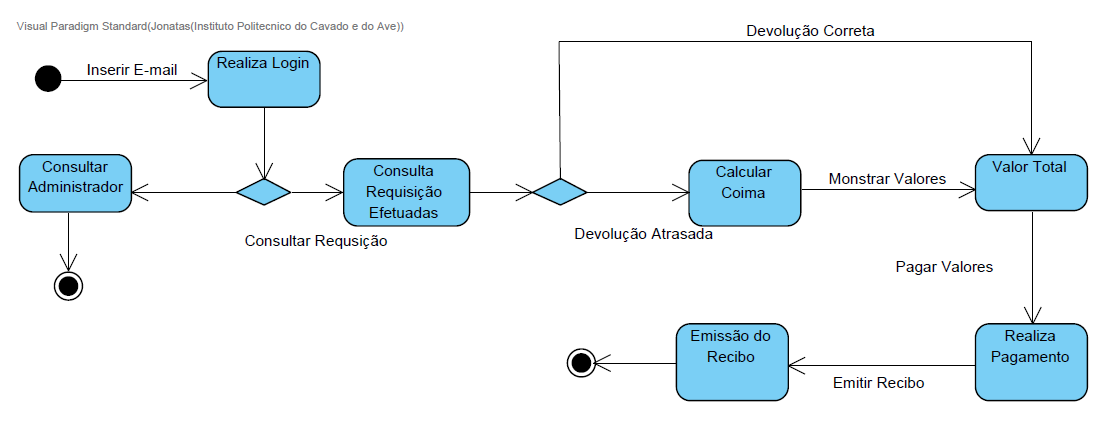
\includegraphics[width=1\linewidth]{./img/Diagrama_E/DE_Pagamento.png}  % largura percentual 
	\caption{\ref{es:252}}
	\label{fig:chap252}
\end{figure}

\par O diagrama de “Pagamento” inicia no estado de "Realiza login", na falha de login o estado altera para “Contactar Administrador” e, após o processo finaliza, no caso de login correto o estado altera “Consulta Requisição Efetuadas” neste momento o usuário terá acesso a todas suas requisições e, no caso de devolução atrasada o estado altera para “Calcular Coima” onde altera o estado para “Valor Total”, deste modo, o sistema altera o estado para “Realiza Pagamento”, após efetuado altera para “Emissão do Recibo”, sendo após finalizado o processo.
